\section{Additional LongMemEval-V2 results}
\label{sec:lmresults}

\subsection{The cell-level sparsity map}
\label{sec:sparsitymap}
Figure~\ref{fig:sparsitymap} draws every one of the $\spCells$ measured cells
of the screened design. It is the cell-level view behind
Figure~\ref{fig:overview}b and Table~\ref*{M-tab:screened} of the main paper.
$\Delta U$ takes exactly three values here, because the reward is binary and
both replicates agree on every cell, so the marks are discrete rather than
shaded. Unmeasured slots are left blank: rows are ragged (at most 9, 9 and 15
cells per memory in the three blocks), and padding them to a rectangle would
spread the same marks over more area. Per drawn square the \textsc{bearing}
rate is $\spBearRate\%$ against $\spRandRate\%$ for \textsc{random}; per padded
area the two would look the same, which is why the figure does not pad.

%%% TikZ figure, drawn from macros/figdata.tex. Included by a section file.
\begin{figure}[t]
\centering
\begin{tikzpicture}[
  font=\scriptsize,
  tk/.style={font=\tiny, text=black!55},
  hd/.style={font=\tiny\bfseries, text=black!80},
  lg/.style={font=\tiny, text=black!60},
  br/.style={draw=black!45, line width=0.35pt},
]
\def\cw{3.5pt}\def\ch{2.1pt}
%% ---- the cells. Order matters: zeros first, so a non-zero mark is never
%% painted over by a neighbouring zero.
\foreach \x/\y in \spZero
  { \fill[teallight!18] (\x pt,\y pt) rectangle +(\cw,\ch); }
\foreach \x/\y in \spNeg
  { \fill[coral] (\x pt,\y pt) rectangle +(\cw,\ch); }
\foreach \x/\y in \spPos
  { \fill[tealdeep] (\x pt,\y pt) rectangle +(\cw,\ch); }
%% ---- stratum headers and the per-block positive rate
\foreach \mi/\nm/\rt/\lo/\hi in {%
    \spBearMid/{\textsc{bearing}}/\spBearRate/\spBearLo/\spBearHi,
    \spCtrlMid/{matched control}/\spCtrlRate/\spCtrlLo/\spCtrlHi,
    \spRandMid/{\textsc{random}}/\spRandRate/\spRandLo/\spRandHi}{
  \node[tk, text=black!75, anchor=south] at (\mi,7pt) {\nm};
  \node[tk, anchor=north] at (\mi,{-\spTotH-1pt})
    {\rt\%\ \,{\tiny[\lo, \hi]}};
}
\node[tk, anchor=north] at (\spBearMid,{-\spTotH-9pt}) {\spBearPos/\spBearN};
\node[tk, anchor=north] at (\spCtrlMid,{-\spTotH-9pt}) {\spCtrlPos/\spCtrlN};
\node[tk, anchor=north] at (\spRandMid,{-\spTotH-9pt}) {\spRandPos/\spRandN};
\node[tk, anchor=north] at (78pt,{-\spTotH-17pt})
  {cells where the memory helped, with Wilson 95\% interval};
%% ---- the memory axis
\draw[br] (-3pt,0pt) -- (-3pt,{-\spTotH});
\node[tk, rotate=90, anchor=south] at (-8pt,{-0.5*\spTotH})
  {\spMems\ memories};
%% ---- legend, raised clear of the stratum headers
\fill[tealdeep] (0pt,20pt) rectangle +(\cw,\ch);
\node[lg, anchor=west] at (5pt,21pt) {helped};
\fill[coral] (30pt,20pt) rectangle +(\cw,\ch);
\node[lg, anchor=west] at (35pt,21pt) {hurt};
\fill[teallight!18] (54pt,20pt) rectangle +(\cw,\ch);
\node[lg, anchor=west] at (59pt,21pt) {no change};
\node[lg, anchor=west] at (95pt,21pt) {(blank $=$ not run)};
\end{tikzpicture}
\caption{\textbf{Utility is sparse over future tasks, and the sparsity is
structured.} One square per \emph{measured} cell --- all $\spCells$ of them,
$\spMems$ memories $\times$ their own future tasks, one representation and
one frozen reader. $\Delta U$ takes exactly three values here, so the marks
are discrete rather than shaded. Only $\spNonzero$ cells move at all:
$\spZeroPct\%$ of measured cells are an exact zero, which is the quantity a
single global memory score has to summarize. The three blocks are the same $\spMems$
memories against bearing, matched-control and unscreened tasks, so the
comparison is paired within memory. Rows are ordered by \textsc{bearing}
count; that arranges the rows but cannot create the block contrast, which is
$\spBearRate\%$ against $\spRandRate\%$ with disjoint Wilson intervals. A row's squares are that memory's own tasks in its
own order, so a \emph{column is not a task}: the blocks span $\spBearTasks$,
$\spCtrlTasks$ and $\spRandTasks$ distinct tasks against widths of 9, 9 and
15. Unrun cells are blank rather than padded --- the rows are ragged, and
padding them would spread the same marks over more area and collapse the
contrast to about $1\times$.}
\label{fig:sparsitymap}
\end{figure}

\subsection{Embedding similarity in detail}
\label{sec:simdetail}
This section holds the detail behind \main{sec:similarity}. Cosine similarity between memory and task, under the pinned embedding model,
is nearly uninformative about $\Delta U$: Spearman $\rho=\simRhoAll$ over all
$\simCells$ cells and $\rho=\simRhoRand$ on unscreened cells alone. The pooled series rises slightly at high
similarity partly because \textsc{bearing} cells concentrate there, and within
\textsc{bearing}, $\rho = +0.164$.

This result is narrower than it looks, for two reasons. First, 96.6\% of the
similarities are computed from a truncated prefix of the memory, and bearing
content sits mostly near the end of a segment: the first $N$ tokens retain it
in 0.7\% of cells against 28.9\% for the last $N$ (\main{sec:repr}).
The embedding therefore mostly never saw the content that matters. Second,
Spearman $\rho$ over an outcome that is exactly zero in $\spZeroPct\%$ of cells
is depressed by ties and is not what a retriever needs, which is to rank the
bearing memory first. We therefore claim only that this embedding
configuration does not track utility, not that embedding similarity cannot.

\subsection{The reader can use the memory}
\label{sec:needle}
We planted a per-cell unique code inside the target memory, in the real
$\sim$27k-token context, and asked the reader for it. The base reader
recovers it in 22 of 22 cells and in 0 of 17 when nothing is planted. Two
larger models also recover 22 of 22 and solve no cell the base reader
missed. The reader can recover planted content at full context length. This makes
a general inability to access the context less likely, but does not rule
out difficulty locating or reasoning over natural evidence. In the two
earlier unscreened arms, accuracy also rises monotonically with how
discriminatively the memory matches the task: $0.1429$, $0.4545$, $0.5000$.

\paragraph{Earlier unscreened arms.}
The same contrast appears in two earlier, unscreened prompt arms, where
bearing was identified afterwards from content alone. On the
$\lfUnsHwN$ and $\lfUnsOffN$ bearing cells of the two arms, mean $\Delta U$ is
$+0.0909$ and $+0.1818$ (2 and 4 net helped cells), against $-0.0066$ and
$-0.0153$ elsewhere; pooled, the difference is $+0.1473$ (permutation
$p = 0.0029$ over 20{,}000 shuffles). These are small samples, and we read them
only as agreeing in sign with the screened design.

\subsection{Length control and budget sweep}
\label{sec:lengthcontrol}
\begin{figure}[t]
\centering
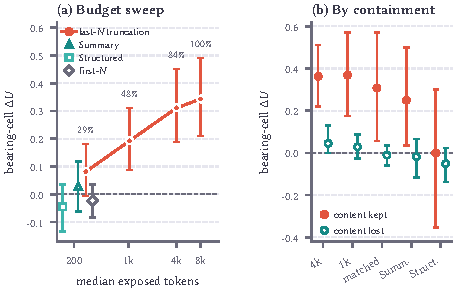
\includegraphics[width=\columnwidth]{fig_lenctl}
\caption{Length-control run on LongMemEval-V2: $\Delta U$ on the
$\lcBearCells$ bearing cells, task-clustered 95\% intervals.
\textbf{(a)}~Raw truncated to its last 4,096 and 1,024 tokens and to each
cell's Summary length (line), against Summary, Structured and the first-$N$
window at that length; percentages give the share of cells whose text still
contains the bearing content. \textbf{(b)}~The same arms split by whether
their text kept the bearing content (filled) or lost it (hollow).}
\label{fig:lenctl}
\Description{Left: bearing-cell utility rising with exposed tokens from about 0.08 at 280 tokens to 0.34 at 8,000, with Summary, Structured and first-N near zero. Right: for each arm, utility near 0.25 to 0.37 when the bearing content is kept and near zero when it is lost, except Structured whose kept estimate is near zero with a wide interval.}
\end{figure}

The length control was frozen before execution. Its extractive arm keeps the
final $N$ tokens of the same source segment, with $N$ set per cell to that
cell's own Summary token count, so it matches Summary's budget without any
model choosing content; a second arm keeps the first $N$ tokens instead, and
last-$N$ versus first-$N$ was registered as the decisive contrast. All three
pre-registered contrasts are computed on the $\lcBearCells$ bearing cells
(two replicate rows each, $\lcPrimaryN$ rows) and clustered over
$\lcBearTasks$ tasks: extractive versus Summary ($\lcPrimary$
$[\lcPrimaryLo, \lcPrimaryHi]$), Raw versus matched extractive ($\lcBudget$
$[\lcBudgetLo, \lcBudgetHi]$), and last-$N$ versus first-$N$ ($\lcEnds$
$[\lcEndsLo, \lcEndsHi]$).

The same run truncated Raw to its last 4,096, 1,024 and 20,000 tokens; the last
equals Raw, since no segment is longer. Table~\ref{tab:sweep} gives each arm's
bearing-cell $\Delta U$, its retention of the bearing content, and $\Delta U$
split by retention. \texttt{make\_lenctl.py} computes every entry from the row
file, whose checksum it verifies against the run manifest, and first checks
that it reproduces the three pre-registered contrasts. The run is not strictly
one session: $\lfLcCacheHits$ responses came from a cache filled minutes
earlier, and $\lcNullRows$ rows with a null reward are excluded, never zeroed.

\begin{table}[t]
\centering\footnotesize
\setlength{\tabcolsep}{2.4pt}
\caption{Length-control run on LongMemEval-V2: bearing-cell $\Delta U$ by arm
($\lcBearCells$ cells, task-clustered 95\% intervals), share of cells whose text
still contains the bearing content, and $\Delta U$ split by whether it does.
Exploratory beyond the three pre-registered contrasts.}
\label{tab:sweep}
\begin{tabular}{@{}lrrrrr@{}}
\toprule
arm & median tokens & kept & $\Delta U$ & $\Delta U\mid$kept & $\Delta U\mid$lost \\
\midrule
Raw (full) & \lcRawTok & \lcRawKept\% & \lcRawM\ [\lcRawLo, \lcRawHi] & \lcRawKM & -- \\
last 4,096 & \lcFourTok & \lcFourKept\% & \lcFourM\ [\lcFourLo, \lcFourHi] & \lcFourKM & \lcFourLM \\
last 1,024 & \lcOneTok & \lcOneKept\% & \lcOneM\ [\lcOneLo, \lcOneHi] & \lcOneKM & \lcOneLM \\
last $N$ (matched) & \lcMatchTok & \lcMatchKept\% & \lcMatchM\ [\lcMatchLo, \lcMatchHi] & \lcMatchKM & \lcMatchLM \\
Summary & \lcSumTok & \lcSumKept\% & \lcSumM\ [\lcSumLo, \lcSumHi] & \lcSumKM & \lcSumLM \\
Structured & \lcStrTok & \lcStrKept\% & \lcStrM\ [\lcStrLo, \lcStrHi] & \lcStrKM & \lcStrLM \\
first $N$ (matched) & \lcFirstTok & \lcFirstKept\% & \lcFirstM\ [\lcFirstLo, \lcFirstHi] & -- & \lcFirstLM \\
\bottomrule
\end{tabular}
\end{table}

\paragraph{Is the kept subset easier?} Retention is a property of the text,
fixed before any outcome, but the cells where a compressed text keeps the
content could still be easier ones. They are not for Summary or the matched
truncation: on the same cells, Raw gains $\lcSelSumKept$ where Summary kept the
content and $\lcSelSumLost$ where it lost it ($\lcSelMatchKept$ and
$\lcSelMatchLost$ for the matched truncation). For Structured the kept cells are
\emph{harder} ($\lcSelStrKept$ against $\lcSelStrLost$), which accounts for
its low kept estimate.

\paragraph{Position.} Target position is identical across all eight arms
within each cell (asserted). Between strata its distribution differs mildly
($\chi^2$ $p = \lcPosChiP$); the position-standardized Raw
\textsc{bearing}$-$control contrast is $\lcPosStd$ against $\lcPosUnadj$
unadjusted, and positive at every position.

\subsection{Formation-cost sensitivity}
\label{sec:reuse}
Formation cost per cell is the writer's tokens divided by the reuse factor
$r$, the number of cells that share one written memory. Our design fixes
$r = \frReuse$, so we recompute exposure efficiency over $r$ from the same
utilities and token counts (Figure~\ref{fig:reuse}). One Summary costs about
$\raFormSum$ writer tokens and one Structured record about $\raFormStr$. On
point estimates Summary overtakes Raw only for $r \gtrsim \raReuseStar$, but
its utility interval spans zero at every $r$, so the crossing point is not
estimated with any precision. Under the sparsity we measure, a memory that
bears on one task may be shown for few others, which pushes $r$ down and
formation cost up. The relevant factor in deployment is exposures per write,
not cells per memory. Input and output tokens are priced identically and prompt
caching is ignored; since output tokens usually cost more, both choices
understate the writer's cost.

\begin{figure}[t]
\centering
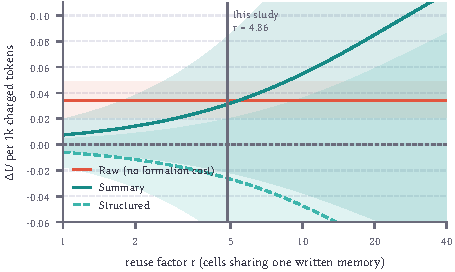
\includegraphics[width=\columnwidth]{fig_reuse}
\caption{Exposure efficiency ($\Delta U$ per thousand charged tokens) against
the reuse factor, on the $\frCells$ representation cells of LongMemEval-V2.
Lines use each representation's paired \textsc{bearing}$-$control effect;
bands use its 95\% interval over memories. Raw has no writer call and does not
depend on $r$. The vertical line marks the reuse factor of this study.}
\label{fig:reuse}
\Description{Line chart of efficiency against reuse factor on a log axis: Raw is flat near 0.034, Summary rises and crosses Raw near r of 5.5 with a wide band spanning zero, Structured is below zero.}
\end{figure}
